\begin{center}
    
\begin{tikzpicture}[x=1em, y=1em]
        \draw[thick] (0,0)--(1,0)--(.5,.866)--(0,0);
    \end{tikzpicture}
    $\cong$
    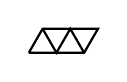
\begin{tikzpicture}[x=1em, y=1em]
        \draw[thick] 
        (0,0)--(2,0)--(2.5,.866)--(.5,.866)--(0,0)
        (.5,.866)--(1,0)--(1.5,.866)--(2,0);
    \end{tikzpicture}
    $\xto{p}$
    
\begin{tikzpicture}[x=.2em, y=.2em, z=-.07em, baseline=0em]
    \draw[thick, black, dashed] 
        (-3,0,0) -- (5,0,0);
    \draw[thick, black]
        (5,0,0)--(0,5,0)
        (0,0,5)--(5,0,0)
        (0,5,0)--(0,0,5)
        (-3,0,0)--(0,5,0)
        (0,0,5)--(-3,0,0);
    \end{tikzpicture}
    $\into$
    
\begin{tikzpicture}[x=.2em, y=.2em, z=-.07em, baseline=0em]
    \draw[thick, black, dashed] 
        (-3,0,0) -- (5,0,0);
    \fill[fill=blue, opacity=0.3]
        (5,0,0)--(0,5,0)--(0,0,5)--(5,0,0);
    \fill[fill=blue, opacity=0.2]
        (-3,0,0)--(0,5,0)--(0,0,5)--(-3,0,0);
    \draw[thick, black]
        (5,0,0)--(0,5,0)
        (0,0,5)--(5,0,0)
        (0,5,0)--(0,0,5)
        (-3,0,0)--(0,5,0)
        (0,0,5)--(-3,0,0);
    \end{tikzpicture}
    $\xto{g} X.$
\end{center}
